% Appendix C

\newpage

\pagebreak
\clearpage
\section{Waspmote Additions}
\subsection{Waspmote Architectural Overview}
\label{AppendixB} % For referencing this appendix elsewhere, use 
\subsubsection{Waspmote Block Diagram}
\begin{figure}[ht]
\centering
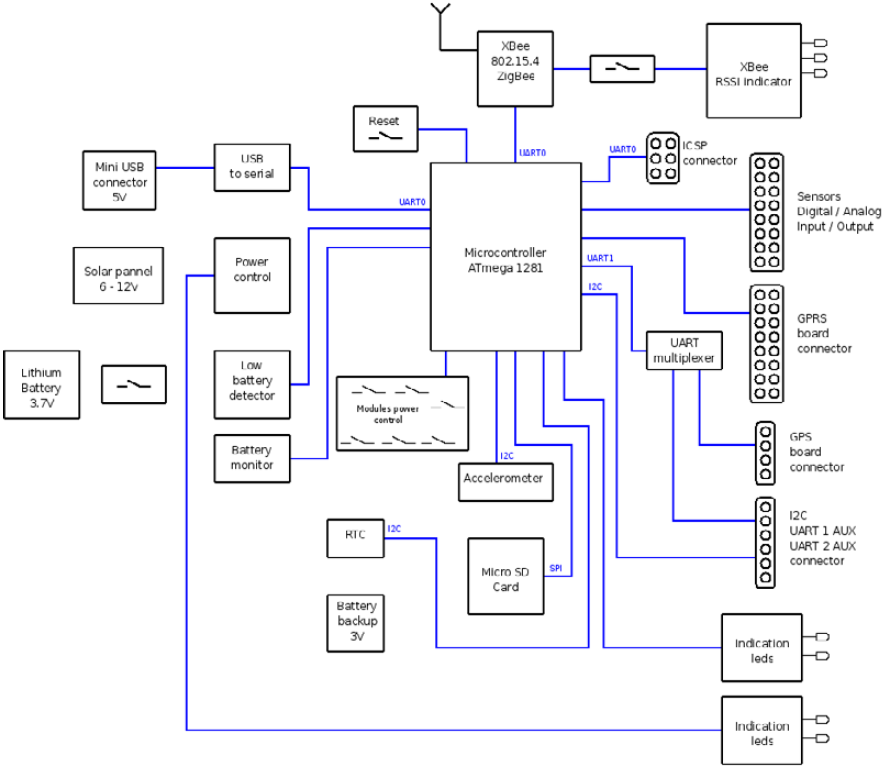
\includegraphics[height=14cm]{block}
\rule{30em}{0.5pt}
\caption{Waspmote block diagram ( $\circlearrowleft$ \ref{fig13} )}
\label{fig:block}
\end{figure}
\vspace{5cm}
\newpage
\clearpage
%-------------------------------------
\pagebreak
\subsubsection{AVR CPU Core Block Diagram}
\vspace{5cm}
\begin{figure}[ht]
\centering
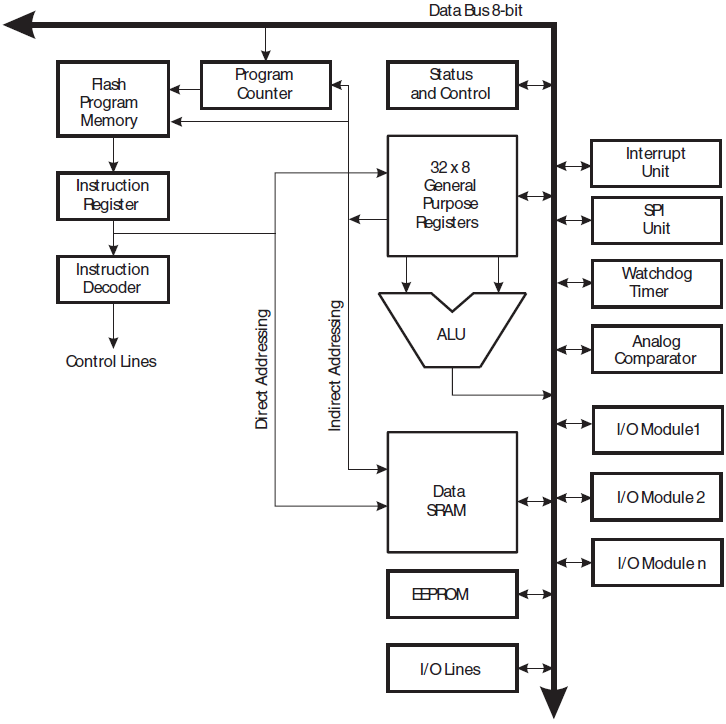
\includegraphics[height=15cm]{architecture}
\caption{AVR CPU block diagram ( $\circlearrowleft$ \ref{fig14} )}
\label{fig:architecture}
\end{figure}
\clearpage
\pagebreak
%-------------------------------------

\subsection{Waspmote Variable Sleep Algorithms}
\label{AppendixC} % For referencing this appendix elsewhere, use 
To support this algorithm also a copy of the original time will be saved and each time the node wakes up it will look for the smallest next time to sleep. This number will be subtracted from the other sleep times in the array. When a value becomes zero it will be restored with its original value and the cycle continues.\\  
This process is fast and simple. However, the main disadvantage is that the node has to write to EEPROM each time it wakes up. According to the Atmel datasheet, the EEPROM of the ATmega1281 has an endurance of at least 100,000 write / erase cycles. The following equation indicates the problem for an interval of 10 seconds:
\begin{equation}
\frac{100000 \mathrm{writes} \cdot 10 \mathrm{s}}{60 \mathrm{s} \cdot 60 \mathrm{min} \cdot 24 \mathrm{h}}= 11,57 \: \mathrm{days} 
\label{eq:1}
\end{equation}
But the processors has 4Kbytes EEPROM on board so we don't have to write to the same place every time. Since EEPROM is written on a 'per cell' basis this can extend the lifetime. Our sensor mask can contain up to 16 values of 2 bytes. This leads to the next result:
\begin{equation}
\frac{100000 \mathrm{writes} \cdot 10 \mathrm{s} \cdot 4\mathrm{KB}}{60 \mathrm{s} \cdot 60 \mathrm{min} \cdot 24 \mathrm{h} \cdot 365\mathrm{days} \cdot 32\mathrm{B}} = 3,96\: \mathrm{years}
\end{equation}
We still must store where the data is stored but this won't cause big problems since we only have to rewrite this cell 125 times:
\begin{equation}
\frac{4\mathrm{KB}}{32\mathrm{B}} = 125 \: \mathrm{locations}
\end{equation}
This supposes however that the EEPROM will not be used for anything else. Below this process is demonstrated.\\
\begin{table}[!hb]
\begin{center}
\begin{tabular}[!hb]{|c|c|c|c|c|}
\hline
\textbf{Sensor[4]} & \textbf{Sensor[3]} & \textbf{Sensor[2]} & \textbf{Sensor[1]} &\textbf{Sensor[0]}\\
\hline
100  & 50 & 35 & 10 & 20\\
\hline
\end{tabular}
\caption{Individual Sensor Sleep Times in seconds}
\label{tab:sleep1}
\end{center}
\end{table}
\begin{table}[!ht]
\begin{center}
\begin{tabular}[!ht]{|c|c|c|c|c|c|c|}
\hline
\textbf{Cycle} & \textbf{Sensor[4]} & \textbf{Sensor[3]} & \textbf{Sensor[2]} & \textbf{Sensor[1]} &\textbf{Sensor[0]} & \textbf{Sleep time}\\
\hline
0 & 100 & 50 & 35 & \textbf{10} & 20 & 10\\
\hline
1 & 90 & 40 & 25 & \textbf{10} & \textbf{10} & 10\\
\hline
2 & 80 & 30 & 15 & \textbf{10} & 20 & 10\\
\hline
3 & 70 & 20 & \textbf{5} & 10 & 10 & 5\\
\hline
4 & 65 & 15 & 25 & \textbf{5} & \textbf{5} & 5\\
\hline
5 & 60 & \textbf{10} & 20 & \textbf{10} & 20 & 10\\
\hline
6 & 50 & 50 & \textbf{10} & \textbf{10} & \textbf{10} & 10\\
\hline
\end{tabular}
\caption{Example of sleep algorithm 1}
\label{tab:sleep2}
\end{center}
\end{table}

\clearpage
\subsection{Practical limitations of Waspmote V1.1}
\subsubsection{IDE and API}
The IDE Libelium offers is very limited, some issues we've experienced are:\\
\begin{itemize}
\item Opening a second or more instance of the IDE sometimes re-opens the previously active files, making it confusing to detect which one you were working in so you end up with two unsaved versions of the same code.
\item Once you start compiling (which takes a lot of time) there's no way to stop it, the stop button does not work.
\item Uploading immediately after compiling will first re-compile it anyway.
\item There is no complete C/C++ support. For example using simple enums is not possible. A workaround is to place the code in additional .h or .cpp files.
\item Auto-completion for the Libelium API functionality would be a great addition.
\end{itemize}
\bigskip
\subsubsection{Hardware aspects}
Also the Waspmote's (V1.1) hardware slows down the programming process:
\begin{itemize}
\item Uploading the code takes a lot of time: 1.5 - 2 minutes.
\item The uploading process fails if:
\begin{itemize}
\item The XBee is present
\item The hibernate jumper is not present when the mote is in hibernate
\item The little power switch has been turned off
\end{itemize}
\end{itemize}
Often you will want to turn off the power switch temporarily to analyse the content of the serial monitor. Especially in pair programming there is often one requirement you forget and the Waspmote does not check for this on beforehand. It will first compile and do as if it is uploading your code, disappointing you at the end of the process.\\
When debugging bigger program these actions come even more annoying. Suppose you are testing a program which measures sensors, sends the values and hibernates. Then you must:
\begin{enumerate}
\item Remove the sensor board
\item Place the hibernate jumper
\item Remove the XBee
\item Upload
\item Place the XBee
\item Remove the hibernate jumper
\item Re-mount the sensor board
\end{enumerate}
And this is not the end of the list. Removing the hibernate jumper causes the Waspmote to crash one out of two times. Resetting the mote has no effect in this case, just keep inserting and removing the little jumper until it agrees with what you want.
\vfill